\subsection{Ley de Amdahl}

\begin{frame}[t]{Ley de Amdahl}
\begin{itemize}
  \item El incremento de rendimiento obtenido usando un modo
        de ejecución más rápido está limitado por la fracción de
        tiempo que se puede usar dicho modo.
  \mode<presentation>{\pause\vfill}
  \item \emph{Speedup} o aceleración:
    \begin{itemize}
      \item Ratio entre el rendimiento mejorado y el rendimiento original.
    \end{itemize}
\end{itemize}
\begin{displaymath}
S = \frac{R(M)}{R(O)}
\end{displaymath}
\begin{displaymath}
S = \frac{T(O)}{T(M)}
\end{displaymath}
\end{frame}

\begin{frame}[t]{Tiempo de ejecución}
\begin{columns}
\begin{column}{0.5\textwidth}
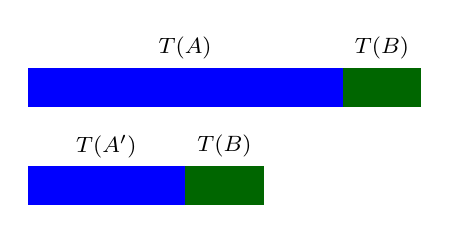
\begin{tikzpicture}
\tikzset{
    etiqueta/.style={text centered, font=\footnotesize} 
}  
\fill(0,1.25) [fill=blue] rectangle (4,1.75);
\fill(4,1.25) [fill=green!40!black] rectangle (5,1.75);
\node[etiqueta] at (2,2) {$T(A)$};
\node[etiqueta] at (4.5,2) {$T(B)$};
\fill(0,0) [fill=blue] rectangle (2,0.5);
\fill(2,0) [fill=green!40!black] rectangle (3,0.5);
\node[etiqueta] at (1,0.75) {$T(A')$};
\node[etiqueta] at (2.5,0.75) {$T(B)$};
\end{tikzpicture}
\end{column}
\pause
\begin{column}{.5\textwidth}
\begin{small}
\begin{displaymath}
F=\frac{T(A)}{T} = \pause
\frac{T(A)}{T(A)+T(B)}
\end{displaymath}
\pause
\begin{displaymath}
S(m)=\frac{T(A)}{T(A')}
\end{displaymath}
\end{small}
\end{column}
\end{columns}
\pause
\begin{small}
\begin{displaymath}
T'=T(A')+T(B) \pause =
\frac{T(A)}{S(m)}+(1-F) \times T
\end{displaymath}
\pause
\begin{displaymath}
T'=\frac{F \times T}{S(m)} + (1-F) \times T
\end{displaymath}
\pause
\begin{displaymath}
T'=T \times \Big[ (1 - F) + \frac{F}{S(m)} \Big]
\end{displaymath}
\end{small}
\end{frame}

\begin{frame}[t]{Ejemplo}
\begin{columns}
\begin{column}{0.5\textwidth}
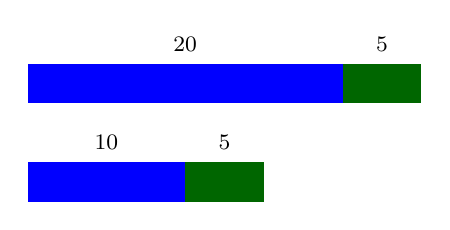
\begin{tikzpicture}
\tikzset{
    etiqueta/.style={text centered, font=\footnotesize} 
}  
\fill(0,1.25) [fill=blue] rectangle (4,1.75);
\fill(4,1.25) [fill=green!40!black] rectangle (5,1.75);
\node[etiqueta] at (2,2) {$20$};
\node[etiqueta] at (4.5,2) {$5$};
\fill(0,0) [fill=blue] rectangle (2,0.5);
\fill(2,0) [fill=green!40!black] rectangle (3,0.5);
\node[etiqueta] at (1,0.75) {$10$};
\node[etiqueta] at (2.5,0.75) {$5$};
\end{tikzpicture}
\end{column}
\pause
\begin{column}{.5\textwidth}
\begin{small}
\begin{displaymath}
F=\frac{20}{20+5}=0.8
\end{displaymath}
\begin{displaymath}
S(m)=\frac{20}{10}=2
\end{displaymath}
\end{small}
\end{column}
\end{columns}
\pause
\begin{small}
\begin{displaymath}
T'=T \times \Big[ (1 - F) + \frac{F}{S(m)} \Big] =
25 \times \Big[ (1-0.8) + \frac{0.8}{2} \Big] = 15
\end{displaymath}
\end{small}
\begin{itemize}
  \item \alert{¡Esto ya lo sabíamos!}
\end{itemize}
\end{frame}

\begin{frame}[t]{Ley de Amdahl}
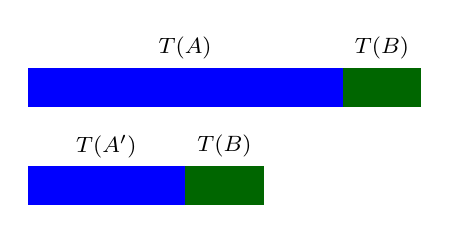
\begin{tikzpicture}
\tikzset{
    etiqueta/.style={text centered, font=\footnotesize} 
}  
\fill(0,1.25) [fill=blue] rectangle (4,1.75);
\fill(4,1.25) [fill=green!40!black] rectangle (5,1.75);
\node[etiqueta] at (2,2) {$T(A)$};
\node[etiqueta] at (4.5,2) {$T(B)$};
\fill(0,0) [fill=blue] rectangle (2,0.5);
\fill(2,0) [fill=green!40!black] rectangle (3,0.5);
\node[etiqueta] at (1,0.75) {$T(A')$};
\node[etiqueta] at (2.5,0.75) {$T(B)$};
\end{tikzpicture}
\begin{small}
\begin{displaymath}
T'=T \times \Big[ (1 - F) + \frac{F}{S(m)} \Big]
\end{displaymath}
\pause
\begin{displaymath}
S=\frac{T}{T'}=\pause
\frac{T}{T \times \Big[ (1 - F) + \frac{F}{S(m)} \Big]} =\pause
\frac{1}{(1 - F) + \frac{F}{S(m)}}
\end{displaymath}
\end{small}
\begin{itemize}
  \item El \textmark{\emph{speedup}} depende \textbf{exclusivamente} de
        la \textgood{fracción de mejora} y el \textgood{speedup de la mejora}.
\end{itemize}
\end{frame}

\begin{frame}[t]{Caso 1}
\begin{itemize}
  \item Un servidor Web distribuye su tiempo en:
    \begin{itemize}
      \item \textmark{Cómputo}: 40%.
      \item \textmark{E/S}: 60%.
    \end{itemize}
  \item Si se sustituye por otra máquina que puede hacer el 
        cómputo 10 veces más rápido, ¿Cuál es el \emph{speedup} global?
\end{itemize}
\mode<presentation>{\pause\vfill}
\begin{block}{Solución}
\begin{displaymath}
S=
\frac{1}{0.6+\frac{0.4}{10}} =
\frac{1}{0.64} =
1.5625
\end{displaymath}
\end{block}
\end{frame}

\begin{frame}[t]{Caso 2}
\begin{itemize}
  \item Una aplicación tiene una parte paralelizable que
        consume el 50\% del tiempo.
    \begin{itemize}
      \item Si se asume que se puede paralelizar esta parte
            completamente con 32 procesadores, ¿cuál será el
            máximo speedup?
    \end{itemize}
\end{itemize}
\mode<presentation>{\pause\vfill}
\begin{block}{Solución}
\begin{displaymath}
S=
\frac{1}{0.5 + \frac{0.5}{32}} =
\frac{1}{0.515625} =
1.9393
\end{displaymath}
\end{block}
\end{frame}

\begin{frame}[t]{Evolución de speedup}
\begin{tikzpicture}
\begin{axis}[xlabel=procesadores,ylabel=speedup, 
minor y tick num=1,
legend style = {
at={(1.02, 1)},
anchor=north west
},
width=0.85\textwidth, height=0.85\textheight,
xmin=0,xmax=128,
ymin=0,ymax=10]
\addplot [domain=1:128,color=red,very thick] {1 / (0.5 + (0.5 / x))};
\addlegendentry{F=0.5}
\addplot [domain=1:128,color=orange,very thick] {1 / (0.4 + (0.6 / x))};
\addlegendentry{F=0.6}
\addplot [domain=1:128,color=green, very thick] {1 / (0.3 + (0.7 / x))};
\addlegendentry{F=0.7}
\addplot [domain=1:128,color=yellow, very thick] {1 / (0.2 + (0.8 / x))};
\addlegendentry{F=0.8}
\addplot [domain=1:128, color=blue, very thick] {1 / (0.1 + (0.9 / x))};
\addlegendentry{F=0.9}
\end{axis}
\end{tikzpicture}
\end{frame}

\begin{frame}[t]{Reflexiones sobre Ley de Amdahl}
\begin{itemize}
  \item Una mejora es más efectiva cuanto más grande es la 
        fracción de tiempo en que ésta se aplica
  \mode<presentation>{\pause\vfill}
  \item Para mejorar un sistema complejo hay que optimizar los elementos 
        que se utilicen durante la mayor parte del tiempo (caso más común).
  \mode<presentation>{\pause\vfill}
  \item Campos de aplicación de las optimizaciones:
    \begin{itemize}
      \item \textmark{Dentro del procesador}: 
            la ruta de datos (data path)
      \item \textmark{En el juego de instrucciones}: 
            la ejecución de las instrucciones más frecuentes
      \item \textmark{En el diseño de la jerarquía de memoria, la programación y la compilación}: 
            hay que explotar la localidad de las referencias.
        \begin{itemize}
          \item El 90\% del tiempo se está ejecutando el 10\% del código.
        \end{itemize}
    \end{itemize}
\end{itemize}
\end{frame}
